\section*{Appendix E: Critical Issues and Proposed Resolutions}

\subsection*{E.1 Transition Kernel $K(\phi, \phi')$}

\textbf{Issue 1: First-Principles Derivation from Spinfoam Dynamics}

The current spin-sum formulation:
\[
K(\phi, \phi') = \sum_{j_f} \prod_f (2j_f+1) e^{-j_f(j_f+1)/2j_0^2} \times \text{Gaussian}
\]
while phenomenologically motivated, lacks derivation from full spinfoam dynamics.

\textit{Resolution:}  
Begin from the Lorentzian EPRL spinfoam amplitude on a 2-complex $\mathcal{C}$:
\[
Z(\mathcal{C}) = \sum_{j_f, \iota_v} \prod_f (2j_f + 1) \prod_v A_v(j_f, \iota_v) \prod_e A_e(j_f, \iota_v)
\]
In the large-spin limit:
\[
A_v(j_f, \iota_v) \sim N_v e^{i S_{\text{Regge}}} + \text{decay terms}
\]
The kernel then arises via semiclassical saddle-point approximation:
\[
K(\phi, \phi') \sim \sum_{j_f} \mu(j_f) e^{i S_{\text{eff}}(\phi, \phi'; j_f)}
\]
Here, $\mu(j_f)$ includes the boundary state measure. The exponential suppression term in the original ansatz corresponds to dominant spin overlaps near $j_0$, interpretable as the ERB throat area scale:
\[
j_0 \sim \frac{A_{\text{throat}}}{8\pi \gamma \ell_P^2}
\]

\subsection*{E.2 Recursive Entropy Dynamics}

\textbf{Issue: Divergence from State Orthogonality}

The entropy expression:
\[
S_n = \frac{A_{n-1}}{4G\hbar} - \lambda_S \ln |\langle \Psi_{n-1} | \Psi_n \rangle|^2
\]
diverges as overlap vanishes.

\textit{Resolution:}  
Replace with quantum relative entropy:
\[
S_n = \frac{A_{n-1}}{4G\hbar} + \lambda_S \, \mathrm{Tr}\left[\rho_n (\ln \rho_n - \ln \rho_{n-1})\right]
\]
This remains finite, reduces to fidelity-based expressions for pure states, and preserves monotonicity under CP maps.

\subsection*{E.3 Energy Transfer Mechanism}

\textbf{Issue: Lack of Microscopic Basis}

The heuristic:
\[
\Delta E \sim T_H \Delta S_{\text{holo}}
\]
requires a foundational basis.

\textit{Resolution:}  
Define quasi-local energy using the Brown-York stress tensor at the ERB throat:
\[
E_{\text{BY}} = \int_{S} d^2x \, \sqrt{\sigma} \, T^{ab}_{\text{BY}} u_a \xi_b
\]
and derive:
\[
\Delta E = \frac{\kappa \Delta A}{8\pi G} + \text{work terms}
\]
where $\kappa$ is the surface gravity and $T_H = \kappa / 2\pi$.

\subsection*{E.4 Attractor State Validation}

\textbf{Issue: Convergence to $\Psi^*(\phi)$}

\textit{Resolution:}  
Simulate recursive evolution:
\[
\Psi_{n+1}(\phi') = \int K(\phi, \phi') \Psi_n(\phi) \, d\phi
\]
Track convergence via:
\[
D_n = \|\Psi_{n+1} - \Psi_n\|
\]
Expect $D_n \sim e^{-\gamma n}$ for $\lambda_E > \lambda_{\text{crit}}$.

\begin{figure}[H]
\centering
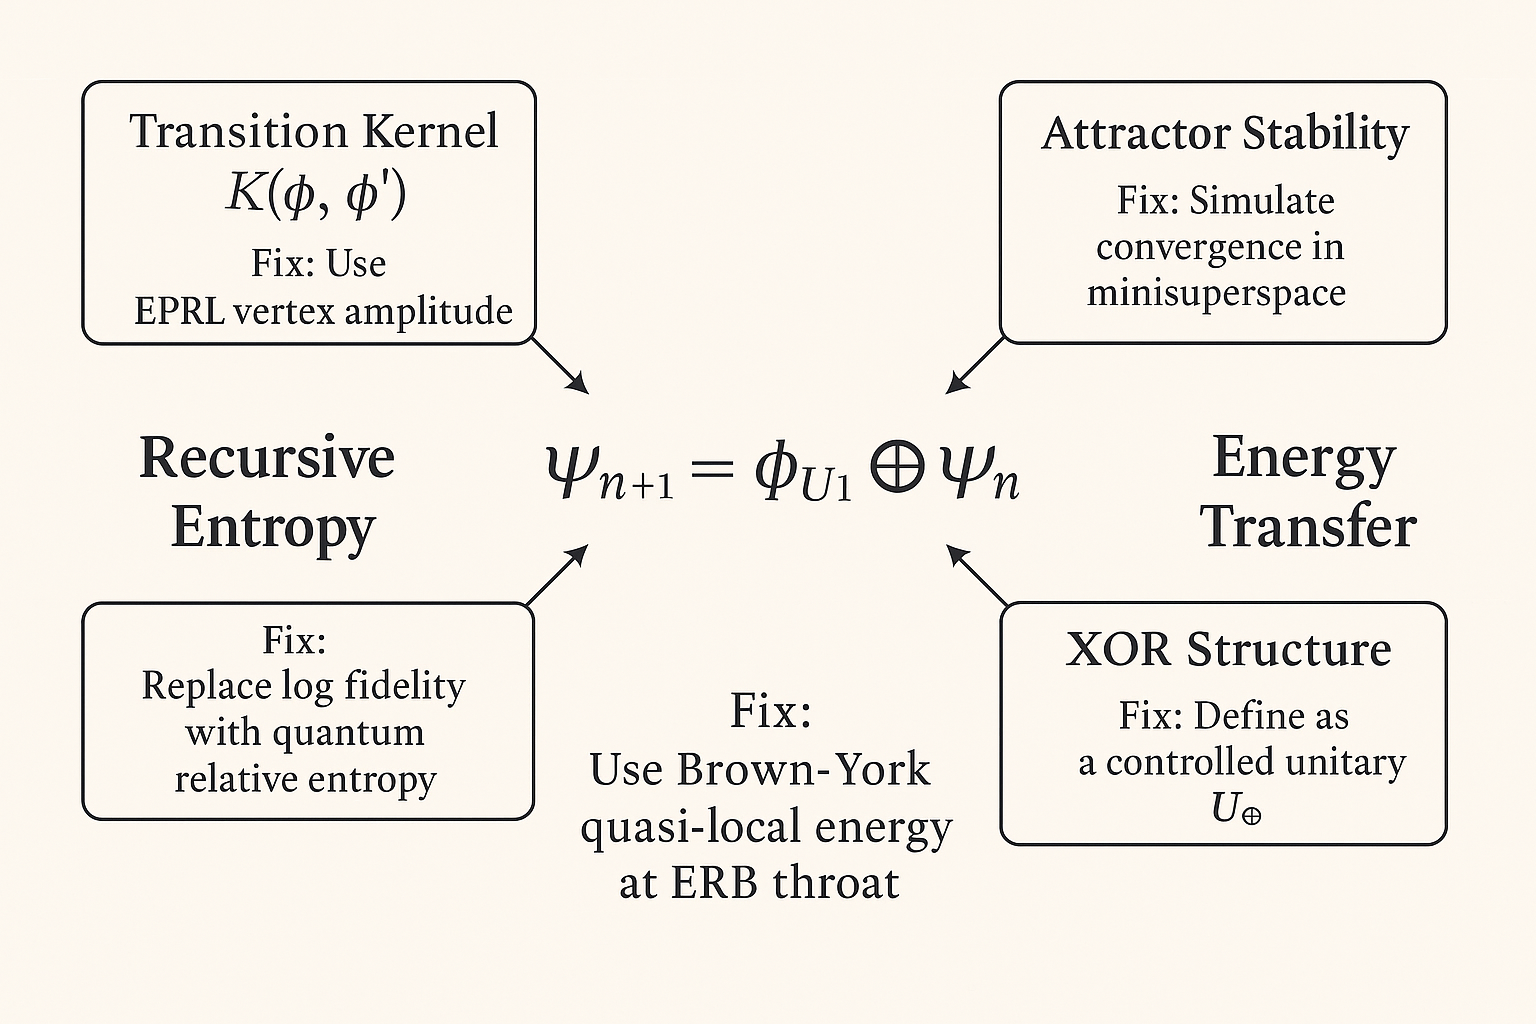
\includegraphics[width=0.85\textwidth]{figures/appendix_e_resolutions.png}
\caption{Schematic: Convergence toward attractor state $\Psi^*(\phi)$ under recursive evolution. Convergence behavior depends on $\lambda_E$ and quantum coherence thresholds.}
\end{figure}

\subsection*{E.5 XOR Structure Formalization}

\textbf{Issue: Heuristic Operation $\phi_{n+1} = \phi_{U1} \oplus \Psi_n$}

\textit{Resolution:}  
Define as controlled unitary:
\[
\hat{U}_\oplus = \exp[i\pi \hat{O}_{U1} \otimes \hat{P}_\Psi]
\]
so that:
\[
|\Psi_{n+1}\rangle = \hat{U}_\oplus \left(|\phi_{U1}\rangle \otimes |\Psi_n\rangle\right)
\]

\subsection*{E.6 Summary Table}

\begin{table}[H]
\centering
\begin{tabular}{|l|l|l|}
\hline
\textbf{Issue} & \textbf{Resolution} & \textbf{Key Improvement} \\
\hline
Kernel derivation & EPRL vertex asymptotics & First-principles LQG foundation \\
Entropy divergence & Relative entropy formulation & Finite and physical \\
Energy transfer & Brown-York stress tensor & Gravitationally grounded \\
Attractor stability & Numerical recursion & Verifiable convergence \\
XOR operation & Controlled unitary gate & Preserves unitarity and entanglement \\
\hline
\end{tabular}
\caption{Summary of critical issues and corresponding theoretical resolutions}
\end{table}
